
\subsection{Aufbau des Nao}
* zu softbank robotics
* allgemeines zur größe, zu den freiheitsgraden und den Sensoren
* Genaueres zu den Sensoren, die gemessen wurden
* Grenzen des Naos
\begin{figure}[htb]
	\centering
	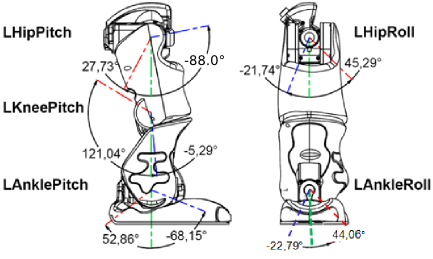
\includegraphics[width=0.7\linewidth]{Bilder/hardware_llegjoint.png}
	\caption{Position und mögliche Winkel der Aktoren des linken Beins. \cite[in /kinematics-data/joints]{nao_docu_dev_guide}}
	\label{hardware_llegjoint}
\end{figure}
\begin{figure}[htb]
	\centering
	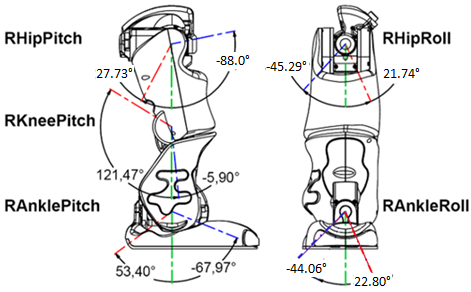
\includegraphics[width=0.7\linewidth]{Bilder/hardware_rlegjoint.png}
	\caption{Position und mögliche Winkel der Aktoren des rechten Beins. \cite[in /kinematics-data/joints]{nao_docu_dev_guide}}
	\label{hardware_rlegjoint}
\end{figure}

\subsection{Magneto-aktive Polymere}

%%% Local Variables:
%%% mode: latex
%%% TeX-master: "main"
%%% End: